% !TEX root = _yoko.tex

% ==========================================
% プロジェクト予稿（1P）の本文
% ==========================================

\section{はじめに}
近年，音楽ストリーミングサービスの普及\red{を経て，楽曲のジャンルは多様化が進んでいる}．
しかし，従来の音楽ジャンル分類手法は楽曲全体を単一のジャンルに分類するものが多く，楽曲内で\red{「ジャンルらしさ」}が時間とともに変化する点を考慮していない．
%
本研究では，楽曲中の時間推移に応じた音楽ジャンル分析・可視化システムの開発を目指す．


\sectionmargin
\section{研究概要}
%従来の音楽ジャンル分類では，楽器構成に着目した研究は比較的少ない．
%しかし楽曲において，楽器構成は聴取者に各ジャンルを印象付ける大きな要因になっていると考える．
%また，多くの楽曲が時間の遷移に伴い楽器構成が変化する．

%そこで
本研究では，音楽ジャンル分析に用いる特徴量を楽器構成に限定し，楽曲の時間の遷移に伴う音楽ジャンルの分析を行う．
%楽曲の類似度分析や可視化\red{については}Maezawaら\cite{maezawa}を、楽器抽出の観点では卓見ら\cite{takumi}\red{の研究に基づいて}を参考に着想と実装を行った。

入力音声（MP3）に対し，機械学習モデルを用いて楽器構成を抽出する\cite{takumi}．
抽出された楽器構成に対してデータベースとの照合を行い，ジャンルの一致率を算出する\cite{maezawa}．
分析結果はグラフとして視覚化し，ジャンルの変化と優勢性を示す．
%
%システムの主な処理は以下のとおりである．

\sectionmargin
\paragraph*{(１)音声データの分割}

%まず，
%入力された音声データを分割する処理を行う．
\red{時間進行に伴って楽曲構成は逐次変化するという仮定のもと，入力音声をセグメントとして分割する．
時間間隔は出力結果に影響するが，筆者の主観で３秒間隔とした．}

%データベースから最も最適であると考えた３秒間隔にセグメントに分割する．

\sectionmargin
\paragraph*{(２)楽器構成の抽出}

音響分類モデルPretrained Audio Neural Networks（PANNs）\cite{PANNs}を用いて，各セグメントの楽器構成を抽出する．
\red{前処理として，}入力音声を32kHzにリサンプリングする．
その後，ノイズ除去や高周波・低周波フィルタの適用，標準偏差に基づく正規化を行った．
%ことで，音響特徴の抽出精度を向上させる工夫を行った．
楽器構成の抽出過程では，反復推論，楽器ごとに閾値を設定することで，楽器抽出精度の向上を図った．


\sectionmargin
\paragraph*{(３)音楽ジャンルの一致率分析}

\red{抽出した楽器\red{構成}情報\red{に基づき}，データベースと照合しながら各ジャンルに対する一致率，すなわち，各ジャンルの中で対象楽曲がジャンル$G$である確率を算出する．}
具体的には，ジャンルごとの楽器出現頻度を用いた重み付けを行い，検出された楽器の出現確率を基にジャンルごとの確率を計算する．
この際，各楽器の出現頻度に対する対数変換を施すことで，対象楽器の寄与度を調整しつつ，一般的な楽器の影響を適切に反映するよう工夫した．

各ジャンル$G$における楽器$i_k$の平均出現確率$P(i_k|G)$を以下の式で定義する．

\begin{equation}
	P(i_k | G) = \frac{1}{N_G} \sum_{j=1}^{N_G} x_{j, i_k}
\end{equation}
%
ここで，$x_{j, i_k}$は楽曲$j$における楽器$i_k$の有無，$N_G$はジャンル$G$に属する楽曲の総数である．
次に，ジャンル$G$の重みは以下のように定義する．

\begin{equation}
	w_{i_k, G} = \log \left( \frac{N_G + 1}{\sum_{j=1}^{N_G} x_{j, i_k} + 1} \right)
\end{equation}
%
各楽器の確率に対して重み$w_{i_k, G}$を指数として乗算することで，楽器の重要度を考慮する．
また，ゼロ除算を防ぐために確率値には小さい平滑化パラメータを適用する．
%
その後，全てのジャンルの確率を合計して正規化を行うことで，音楽ジャンルの一致率を計算する．

\sectionmargin
\paragraph*{(４)可視化}

各セグメントにおけるジャンル\red{一致率}の分布を可視化する（図\ref{fig:EMPIREs}）．
%各セグメントごとのジャンル確率を棒グラフとして表示し，
ジャンル\red{別}に色分けをし，ジャンルの優勢性\red{が見やすいようにした．}%を明確に示すよう設計した．


\sectionmargin
\section{検証}
SnowManの「EMPIRE」\cite{EMPIRE}冒頭1分19秒を使用して本システムの検証を行った．
%
この楽曲は，モーツァルト作曲「交響曲第25番ト短調 K.183」の第一楽章を\red{引用，編曲}した楽曲であり，classicのオーケストラサウンドとjazzの要素が時間\red{推移}に伴い混在する楽曲となっている．

システムによる分析結果と楽曲の構成が一致していることを確認し，提案手法の有効性を評価した．
%
一方で、backing vocalやoboe，violaの抽出が困難である課題も見られた．

\begin{figure}[tb]
	\centering
	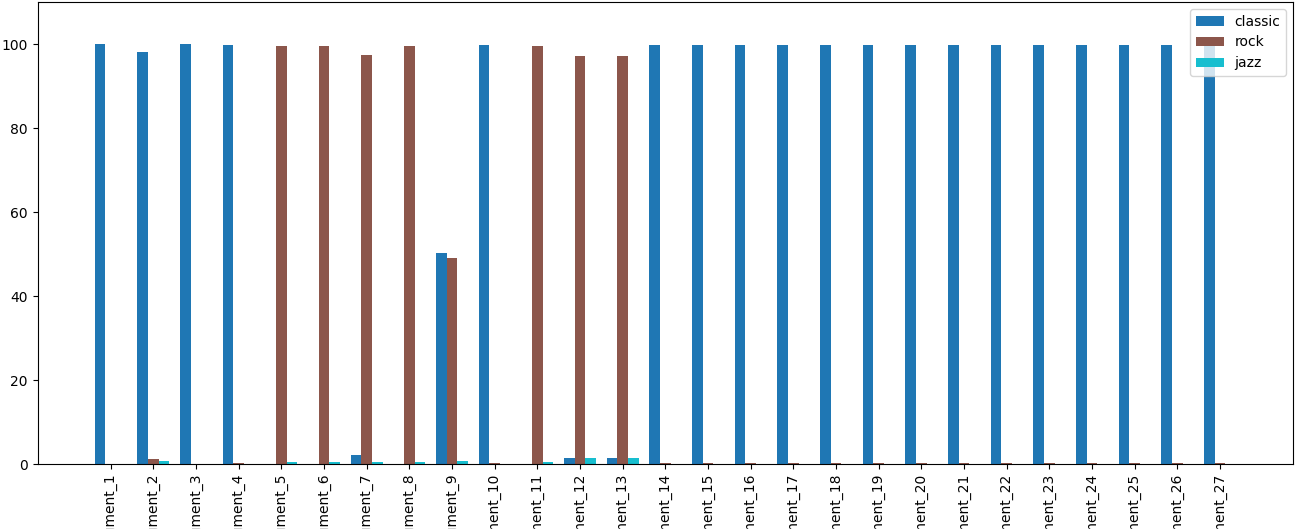
\includegraphics[width=\hsize]{fig/fig36-EMPIREs.png}
	\caption{「EMPIRE」冒頭部分の音楽ジャンル一致率\\（水色：classic，茶色：rock）}
	\label{fig:EMPIREs}
\end{figure}


\sectionmargin
\section{今後の課題と展望}
本研究では，楽曲中の時間推移に伴う音楽ジャンルの変化を分析・可視化するシステムを提案し，検証を行った．
％
時間経過に伴うジャンルの変化が明確に示され，本システムが音楽ジャンルの動的分析に有効であることが確認された．
一方で、backing vocalやoboeなど，一部の楽器の識別が困難である課題も見られた．




